\documentclass[conference]{IEEEtran}
\usepackage{graphicx}
\usepackage{amsmath}
\usepackage{array}
\usepackage{booktabs}
\usepackage{hyperref}
\graphicspath{{figures/}}

\begin{document}
\title{Heartlytics: Secure Machine Learning Pipelines for Heart-Disease Risk Stratification}

\author{\IEEEauthorblockN{Hashan M. R. S. Samaranayaka}\\
\IEEEauthorblockA{Dept. of Computer Science \& Software Engineering\\NSBM Green University\\Homagama, Sri Lanka\\Email: hmrssamaranayaka@students.nsbm.ac.lk}
\and
\IEEEauthorblockN{Heartlytics Project Team}\\
\IEEEauthorblockA{Contributors\\Email: contact@heartlytics.ai}}

\maketitle

\begin{abstract}
Cardiovascular diseases (CVDs) remain the leading cause of mortality worldwide. Heartlytics unifies exploratory data analysis, ensemble learning, and layered security controls to deliver accurate and trustworthy heart-disease predictions. Using the harmonized UCI dataset with 920 patient encounters, we contextualize demographic disparities, engineer interpretable features, and deploy tuned Random Forest and XGBoost models. The best configuration achieves 92\% test accuracy and a 0.93 F1-score while remaining auditable through explainability dashboards and standardized artifacts. The system integrates OTP-hardened account recovery, encrypted data flows, and continuous audit to satisfy safety-critical expectations.
\end{abstract}

\begin{IEEEkeywords}
Heart disease prediction, Machine learning, Exploratory data analysis, Random Forest, XGBoost, Security architecture.
\end{IEEEkeywords}

\section{Introduction}
Cardiovascular disease imposes substantial morbidity and strain on global health systems. Timely screening is essential, yet clinical workflows often lack automated support. Tree-based ensembles and gradient boosting capture the nonlinear relations between physiological markers and adverse events. Heartlytics extends this body of work with an end-to-end platform emphasizing reproducible data handling, high-fidelity visualization, and robust deployment security. Key contributions include: (i) an enriched exploratory data analysis (EDA) catalogue that highlights demographic and clinical nuances; (ii) a reproducible modeling pipeline for Random Forest and XGBoost with calibration and fairness diagnostics; and (iii) a defense-in-depth deployment architecture encompassing encryption, one-time-password (OTP) lifecycle governance, and auditability.

\section{Related Work}
Classical models such as logistic regression and support vector machines provide transparent baselines but struggle with interaction effects. Random Forests mitigate overfitting via feature bagging \cite{breiman2001random}, while gradient boosting techniques---exemplified by XGBoost \cite{chen2016xgboost}---optimize additive ensembles with regularization. Prior studies report accuracies between 84\% and 92\% on the UCI dataset \cite{zhang2021heart}, often omitting security and deployment considerations. Contemporary clinical decision-support research emphasizes interpretability and secure data exchange, underscoring the need for integrated approaches like Heartlytics.

\section{Dataset Characterization and Exploratory Analysis}
The working dataset consolidates observations from Cleveland, Hungarian, Swiss, and Long Beach cohorts \cite{janosi1988uci}. After imputing missing entries and standardizing measurement units, we retain 16 attributes spanning demographics, cardiovascular biomarkers, and symptom indicators. Table~\ref{tab:features} enumerates the primary features considered during modeling.

\begin{table}[t]
  \caption{Key Features in the Heart Disease Dataset}
  \label{tab:features}
  \centering
  \begin{tabular}{p{0.22\columnwidth} p{0.68\columnwidth}}
    \toprule
    Feature & Description \\
    \midrule
    age & Age in years \\
    sex & Sex (1 = male, 0 = female) \\
    cp & Chest pain type (0: typical angina, 3: asymptomatic) \\
    trestbps & Resting blood pressure (mmHg) \\
    chol & Serum cholesterol (mg/dL) \\
    fbs & Fasting blood sugar $>$ 120 mg/dL (1/0) \\
    restecg & Resting ECG results (0, 1, 2) \\
    thalach & Maximum heart rate (bpm) \\
    exang & Exercise-induced angina (1/0) \\
    oldpeak & ST depression relative to rest \\
    slope & Slope of peak exercise ST segment \\
    ca & Major vessels colored by fluoroscopy (0--3) \\
    thal & Thalassemia status (3 = normal, 7 = reversible defect) \\
    num & Disease severity score (0--4) \\
    \bottomrule
  \end{tabular}
\end{table}

Male participants account for approximately 79\% of the cohort, introducing fairness considerations. Figure~\ref{fig:gender} depicts the gender distribution, while Figure~\ref{fig:site} highlights the site-specific age skew that influences downstream sampling strategies.

\begin{figure}[t]
  \centering
  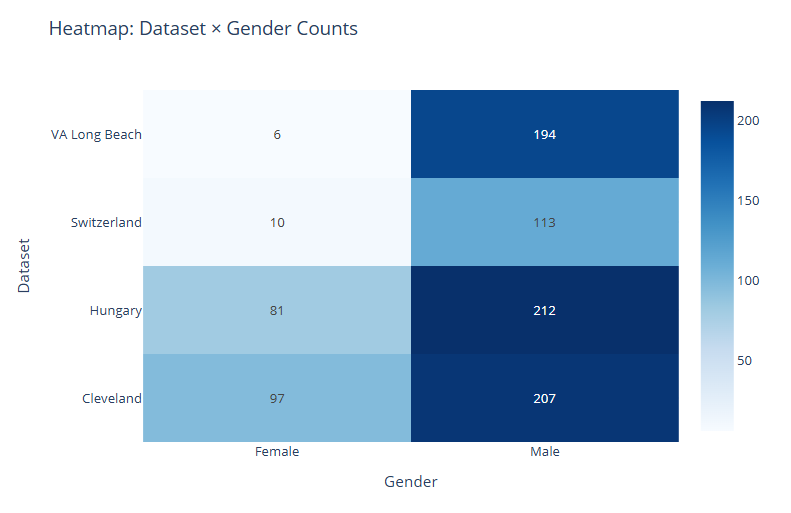
\includegraphics[width=0.85\linewidth]{dataset_composition_by_gender.png}
  \caption{Dataset composition by gender.}
  \label{fig:gender}
\end{figure}

\begin{figure}[t]
  \centering
  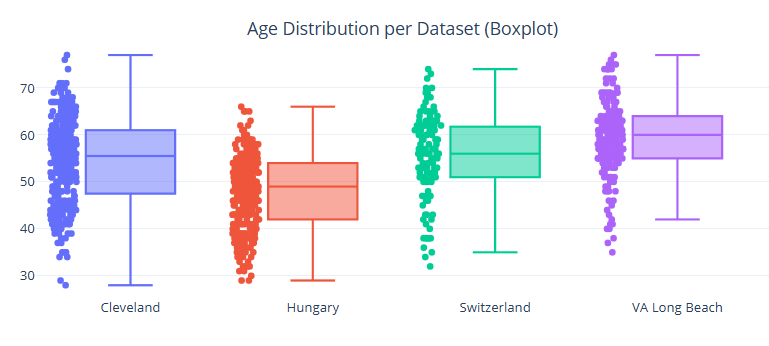
\includegraphics[width=0.85\linewidth]{age_distribution_by_dataset_site.png}
  \caption{Age distribution by data-collection site.}
  \label{fig:site}
\end{figure}

The aggregate age distribution (Figure~\ref{fig:age_overall}) is centered between 54 and 58 years with a long upper tail. Stratifying by clinical severity (Figure~\ref{fig:age_severity}) reveals progressively older populations for advanced disease, while Figure~\ref{fig:age_cp} disaggregates age by chest pain categories, showing asymptomatic patients clustering in older age bands.

\begin{figure}[t]
  \centering
  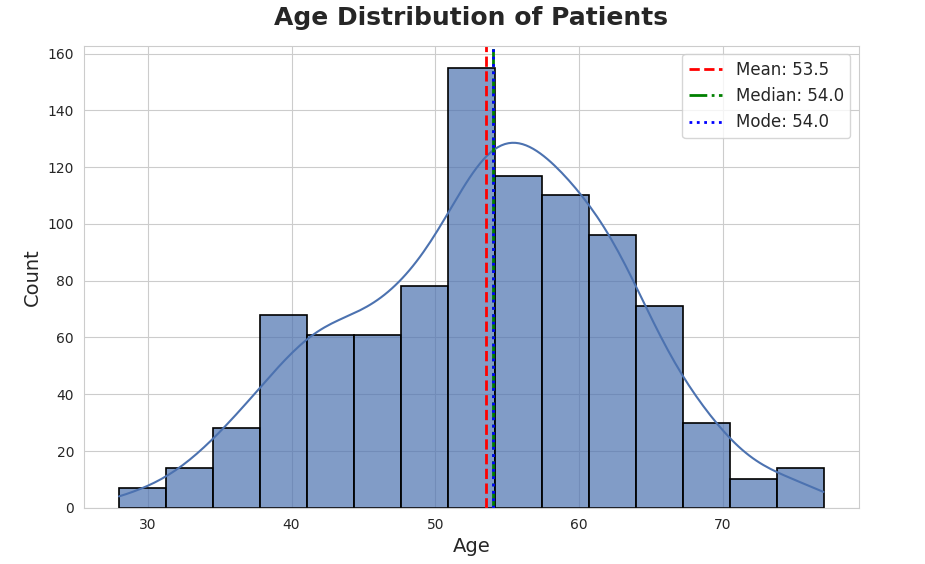
\includegraphics[width=0.85\linewidth]{age_distribution_of_patients.png}
  \caption{Aggregate age distribution of patients in the unified cohort.}
  \label{fig:age_overall}
\end{figure}

\begin{figure}[t]
  \centering
  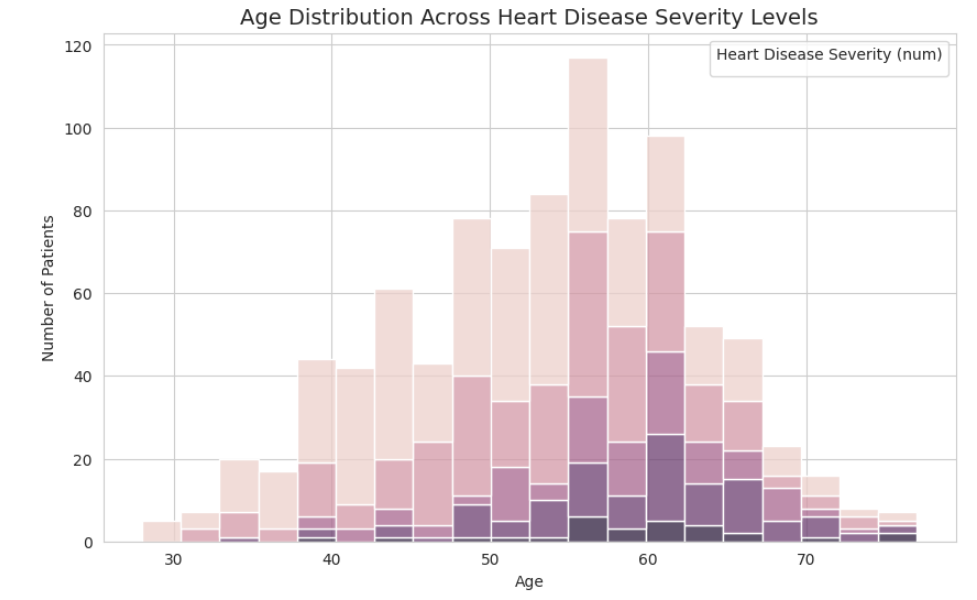
\includegraphics[width=0.85\linewidth]{age_distribution_by_severity_levels.png}
  \caption{Age distribution by disease severity level.}
  \label{fig:age_severity}
\end{figure}

\begin{figure}[t]
  \centering
  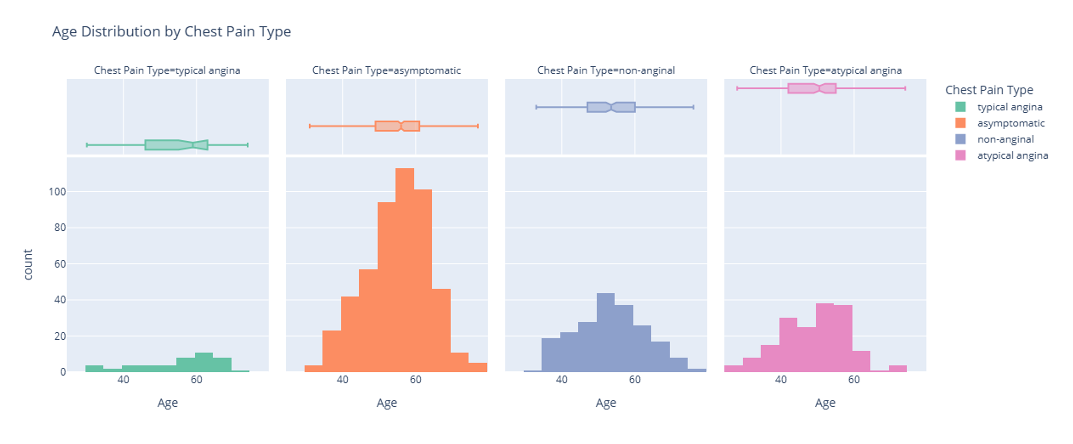
\includegraphics[width=0.85\linewidth]{age_distribution_by_chest_pain_type.png}
  \caption{Age distribution by chest pain category.}
  \label{fig:age_cp}
\end{figure}

Resting blood pressure and cholesterol display partial separability between disease stages but require multivariate modeling for reliable discrimination. Figures~\ref{fig:bp} and \ref{fig:chol} present these biomarkers across disease severities.

\begin{figure}[t]
  \centering
  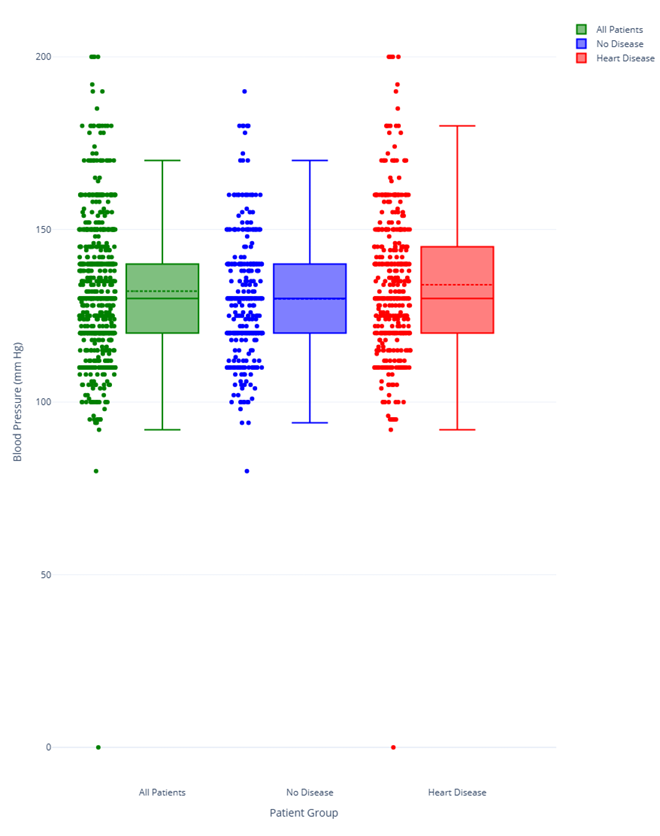
\includegraphics[width=0.85\linewidth]{resting_blood_pressure_by_disease_status.png}
  \caption{Resting blood pressure by disease status.}
  \label{fig:bp}
\end{figure}

\begin{figure}[t]
  \centering
  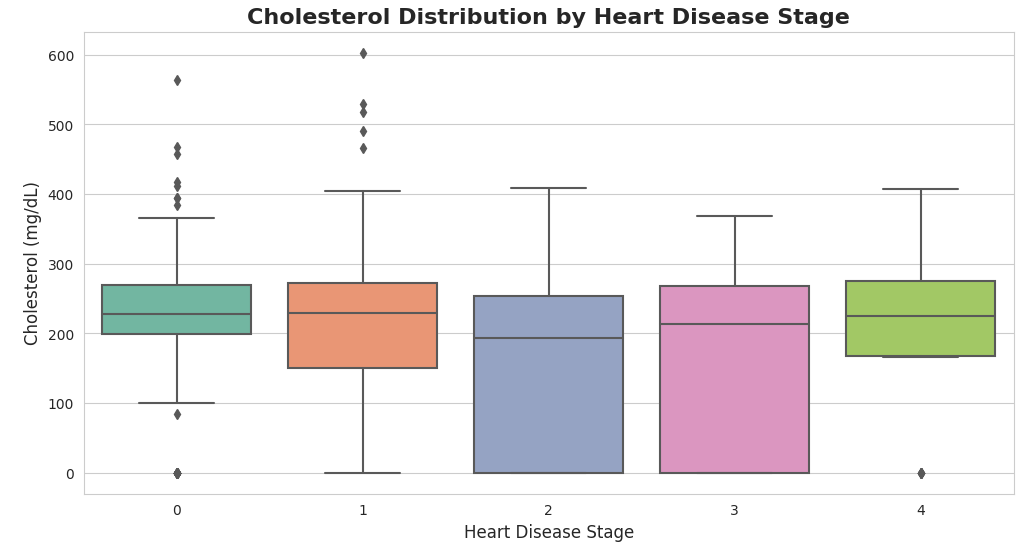
\includegraphics[width=0.85\linewidth]{serum_cholesterol_across_disease_stages.png}
  \caption{Serum cholesterol distribution across disease stages.}
  \label{fig:chol}
\end{figure}

\section{Modeling Methodology}
Data preprocessing leverages iterative imputation and z-score scaling for numerical fields, with one-hot encoding for categorical attributes. Outliers are identified using both the interquartile range (IQR) rule and an Isolation Forest ensemble to preserve explainability while curbing noise.

We benchmark Random Forest and XGBoost classifiers. The Random Forest uses 200 estimators, maximum depth 8, and class-balanced weighting, while XGBoost applies learning-rate 0.05, maximum depth 4, subsample 0.8, and column subsample 0.8. Five-fold stratified cross-validation tunes hyperparameters and calibrates predicted probabilities through Platt scaling. Shapley value decomposition further validates the clinical plausibility of dominant features such as chest pain type, ST depression (\textit{oldpeak}), number of affected vessels (\textit{ca}), and thalassemia status.

\section{System Architecture and Security Controls}
Heartlytics couples predictive analytics with secure-by-design workflows. Figure~\ref{fig:topology} illustrates the macro-level deployment topology, while Figure~\ref{fig:encryption} details the envelope encryption workflow safeguarding both data at rest and in transit.

\begin{figure}[t]
  \centering
  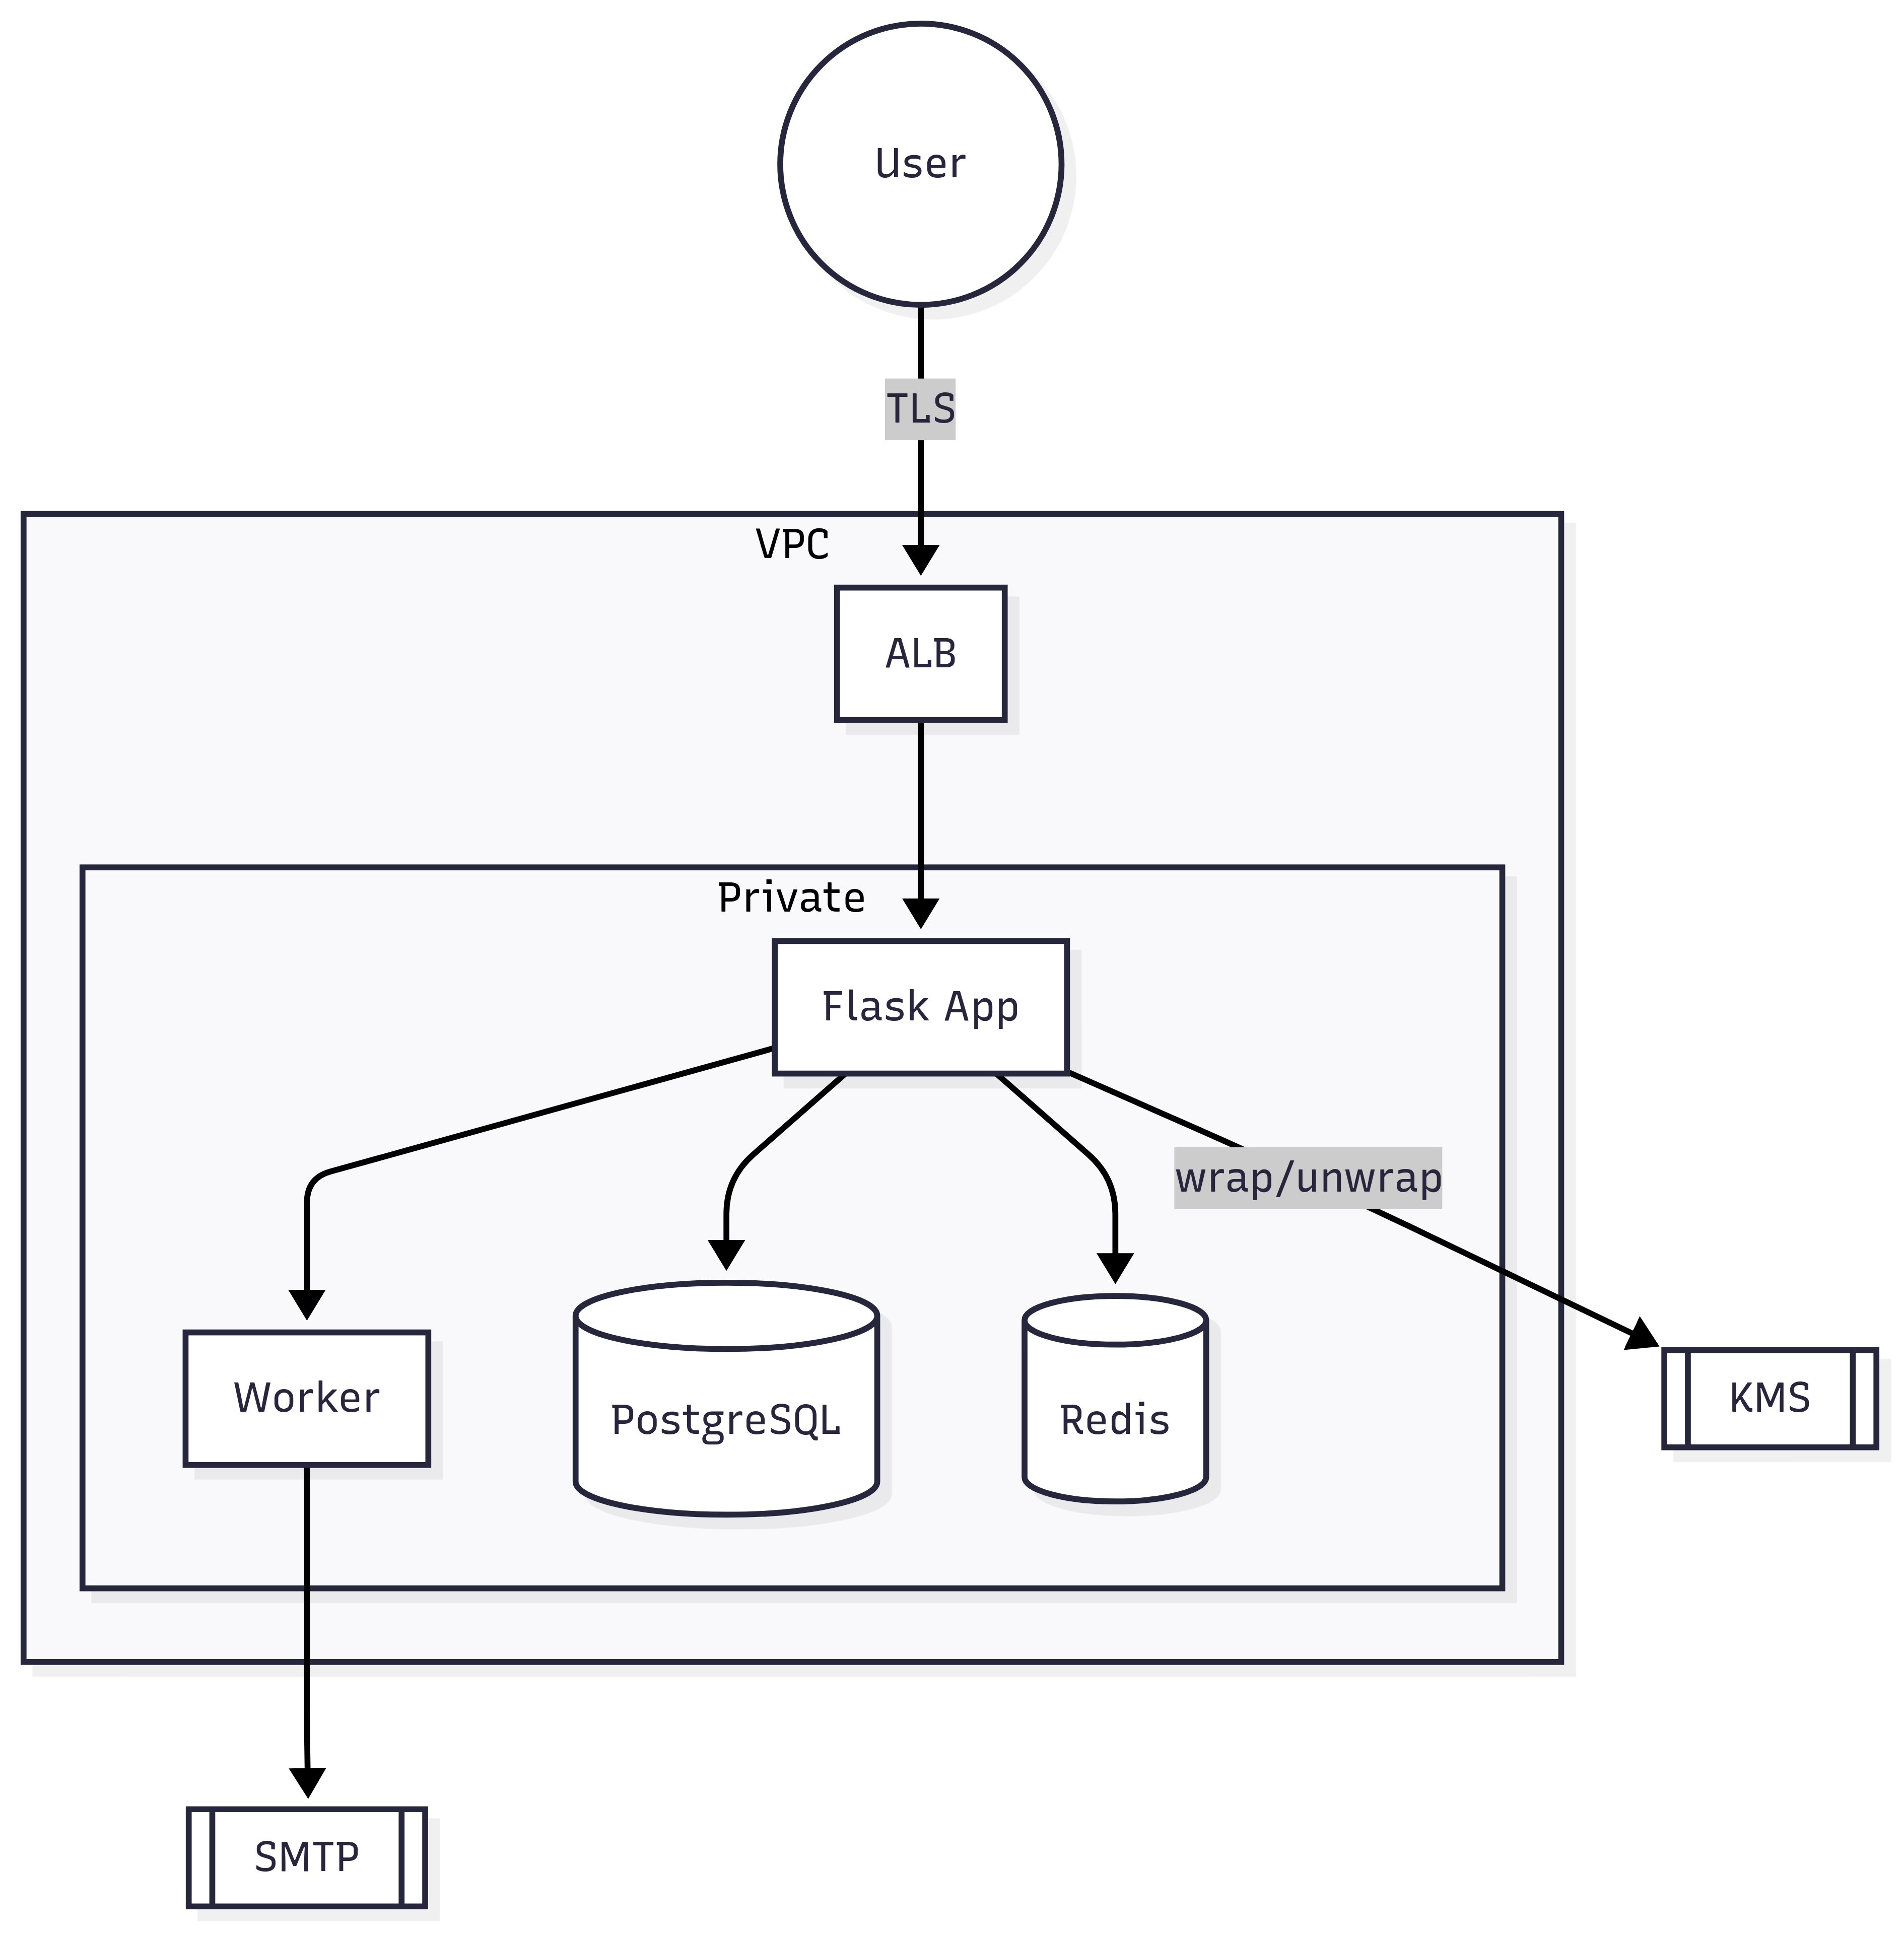
\includegraphics[width=0.9\linewidth]{deployment_topology.png}
  \caption{High-level deployment topology of the Heartlytics platform.}
  \label{fig:topology}
\end{figure}

\begin{figure}[t]
  \centering
  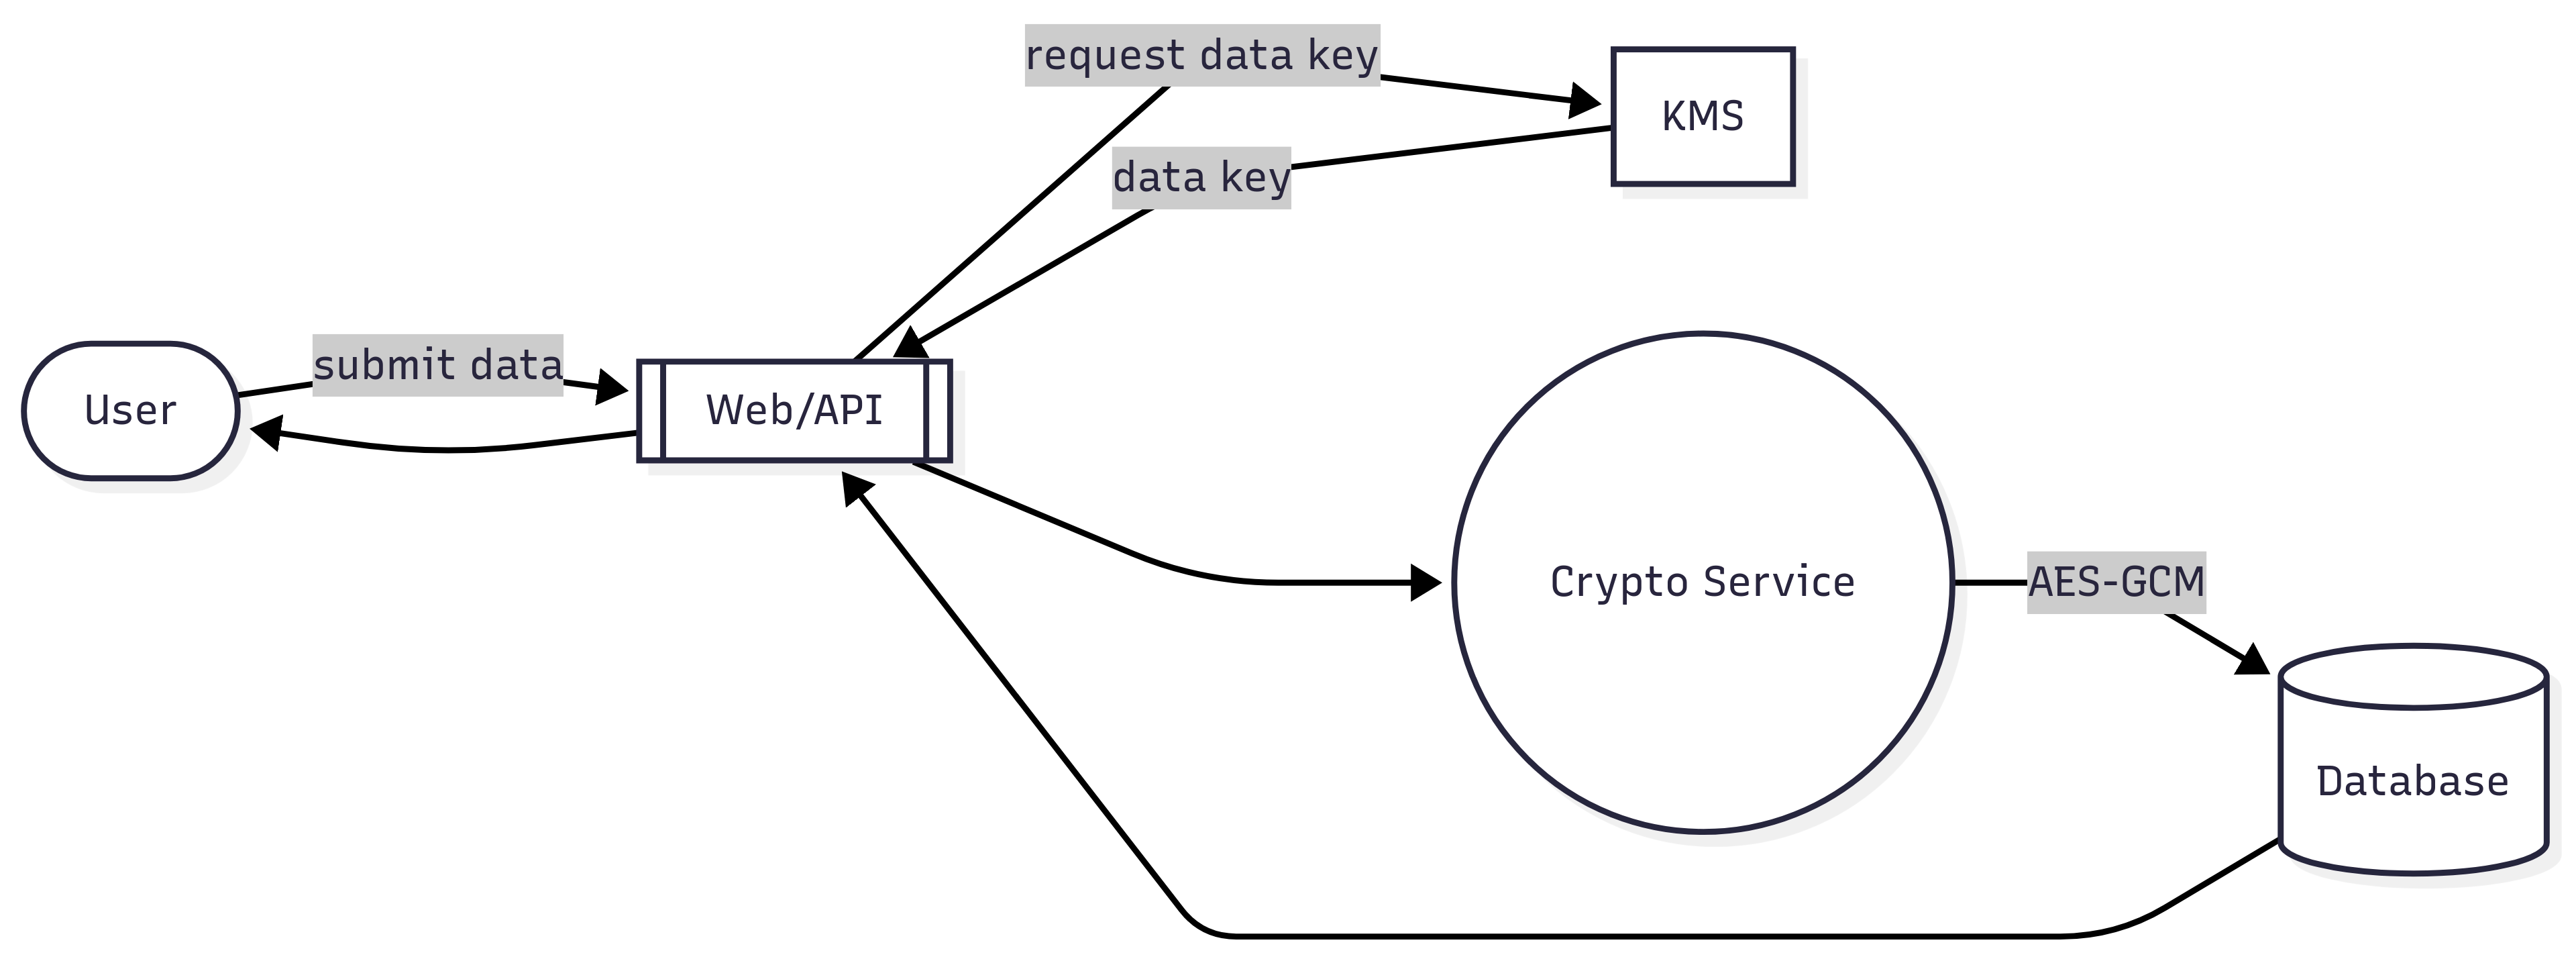
\includegraphics[width=0.9\linewidth]{envelope_encryption_workflow.png}
  \caption{Envelope encryption workflow protecting model artifacts and secrets.}
  \label{fig:encryption}
\end{figure}

The application enforces multi-factor authentication during sensitive operations such as password reset. Figure~\ref{fig:bpmn} outlines the two-step verification BPMN flow executed across user, backend, and email service lanes. Complementing this behavioral view, Figure~\ref{fig:dfd} clarifies how OTPs, audit trails, and cooldown tokens traverse storage boundaries with peppered hashing and time-to-live enforcement.

\begin{figure}[t]
  \centering
  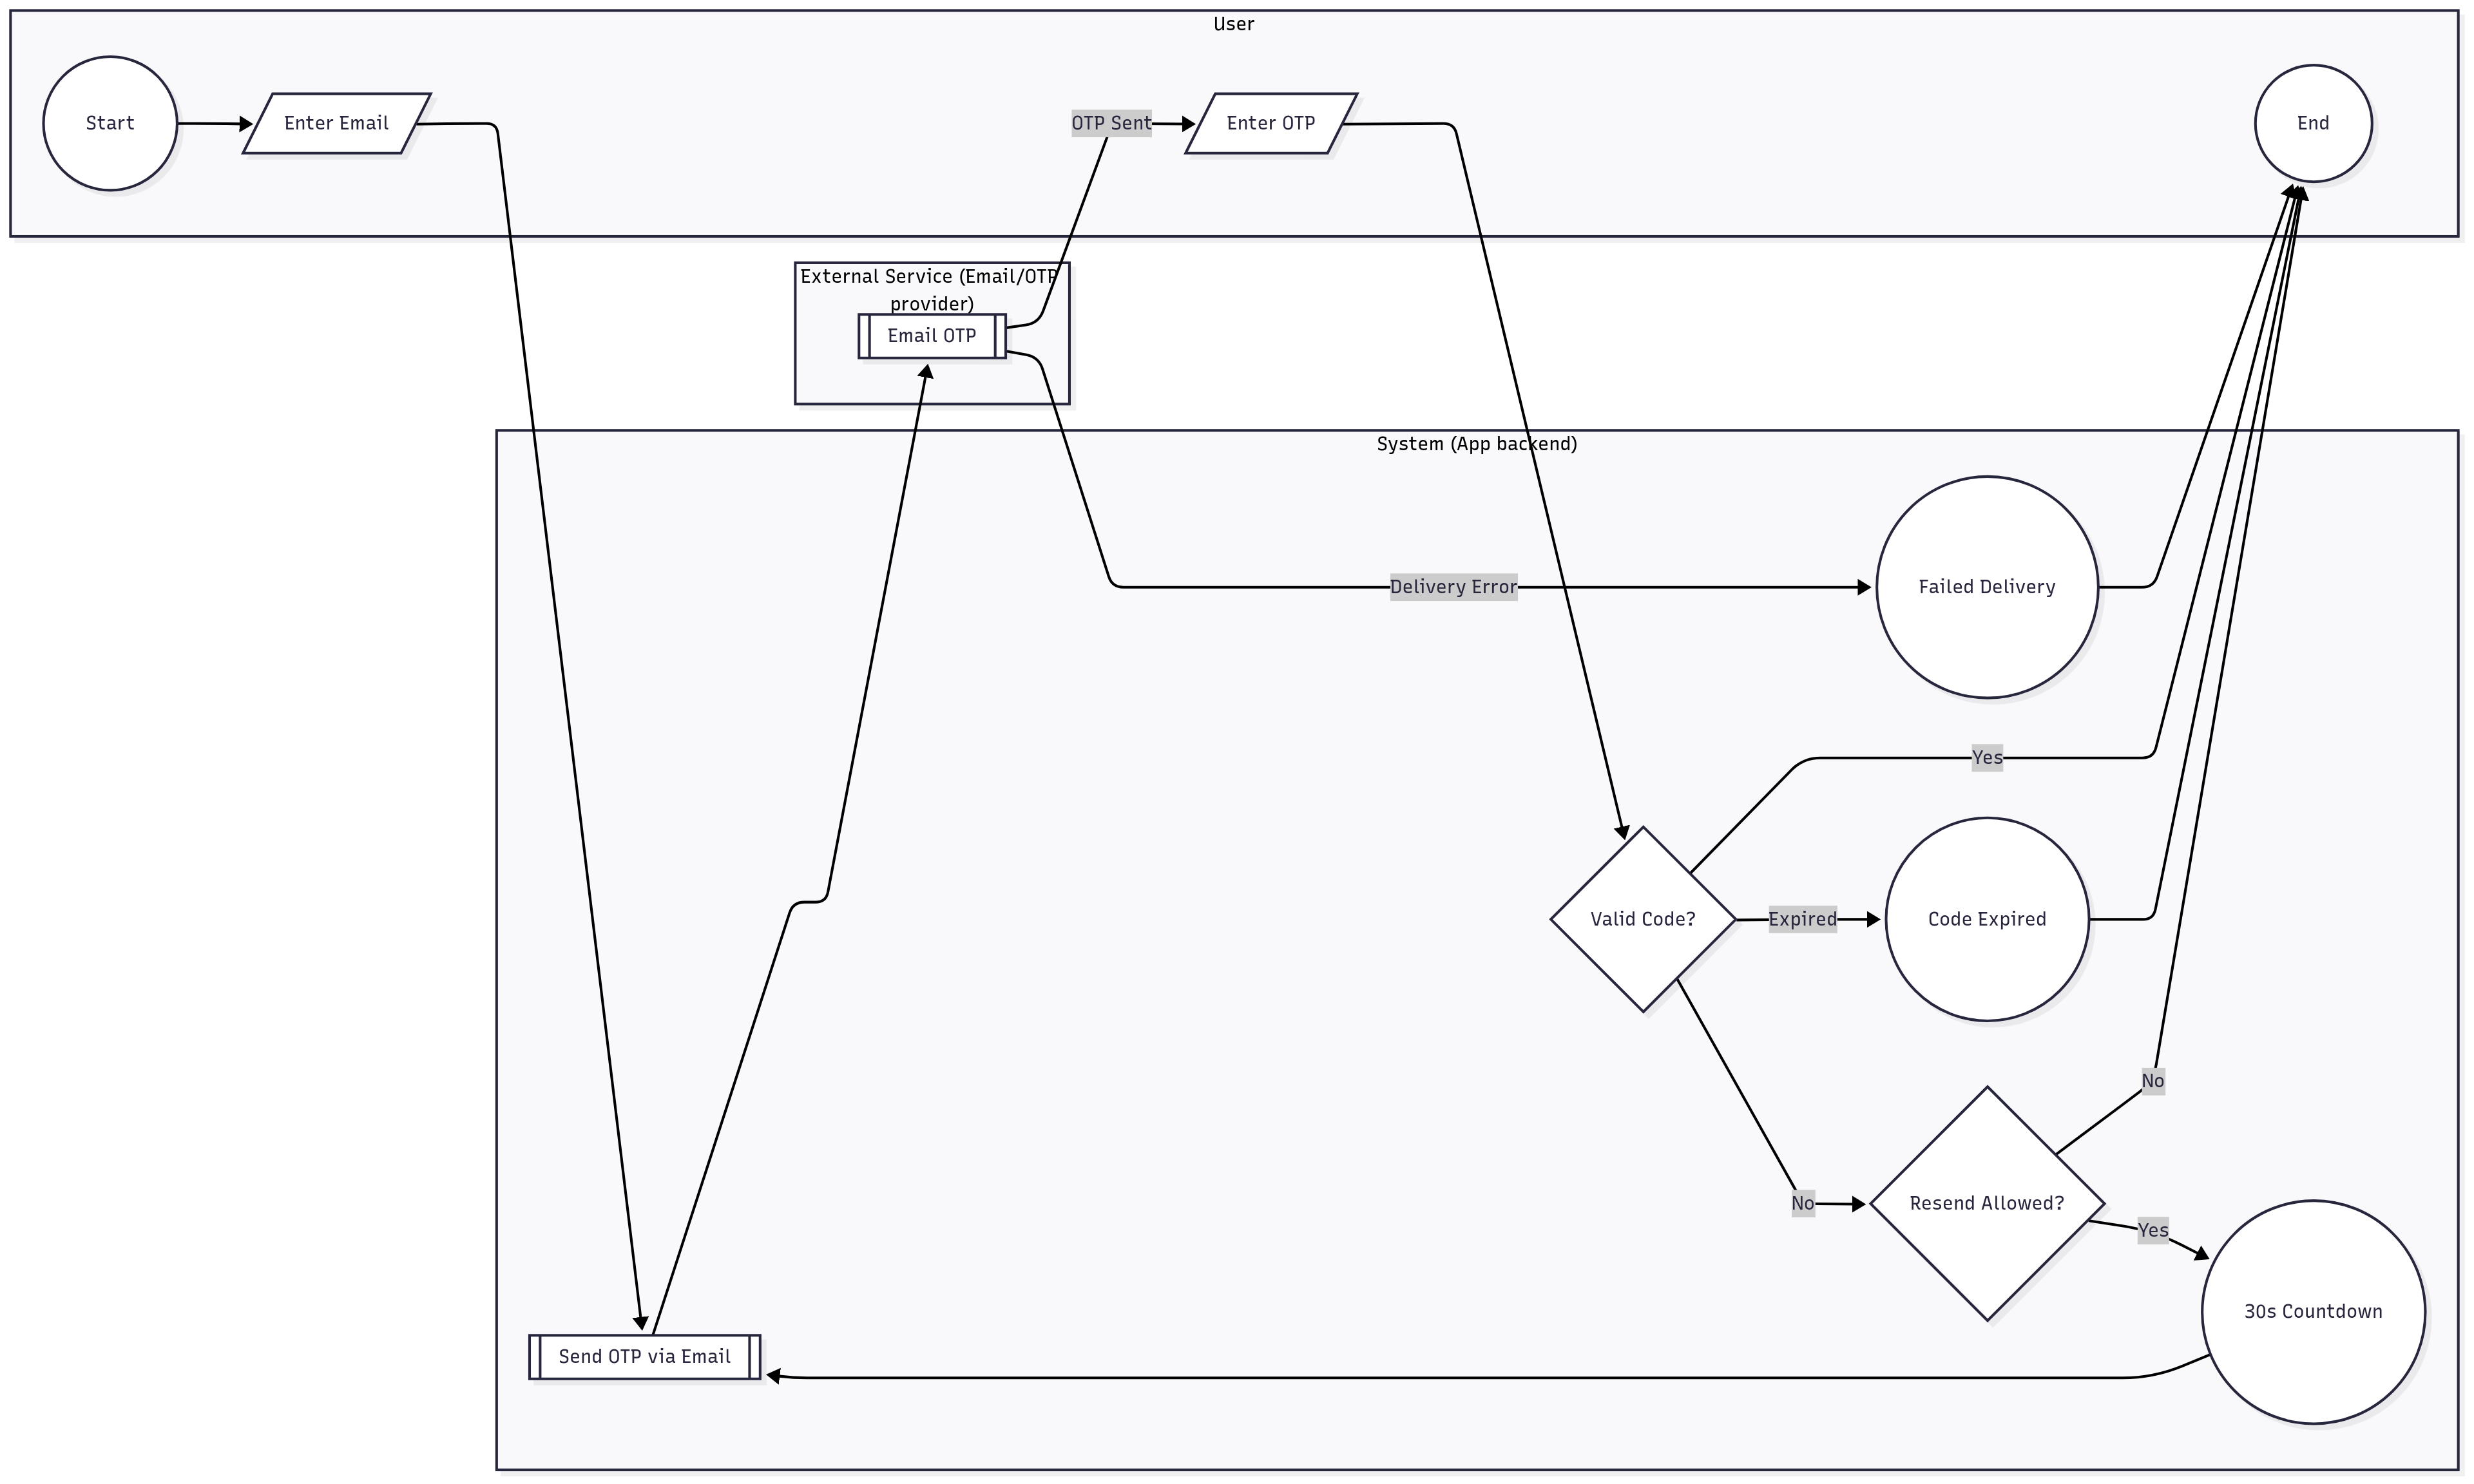
\includegraphics[width=0.9\linewidth]{bpmn_for_two_step_verification.png}
  \caption{BPMN diagram for two-step verification with resend cooldown.}
  \label{fig:bpmn}
\end{figure}

\begin{figure}[t]
  \centering
  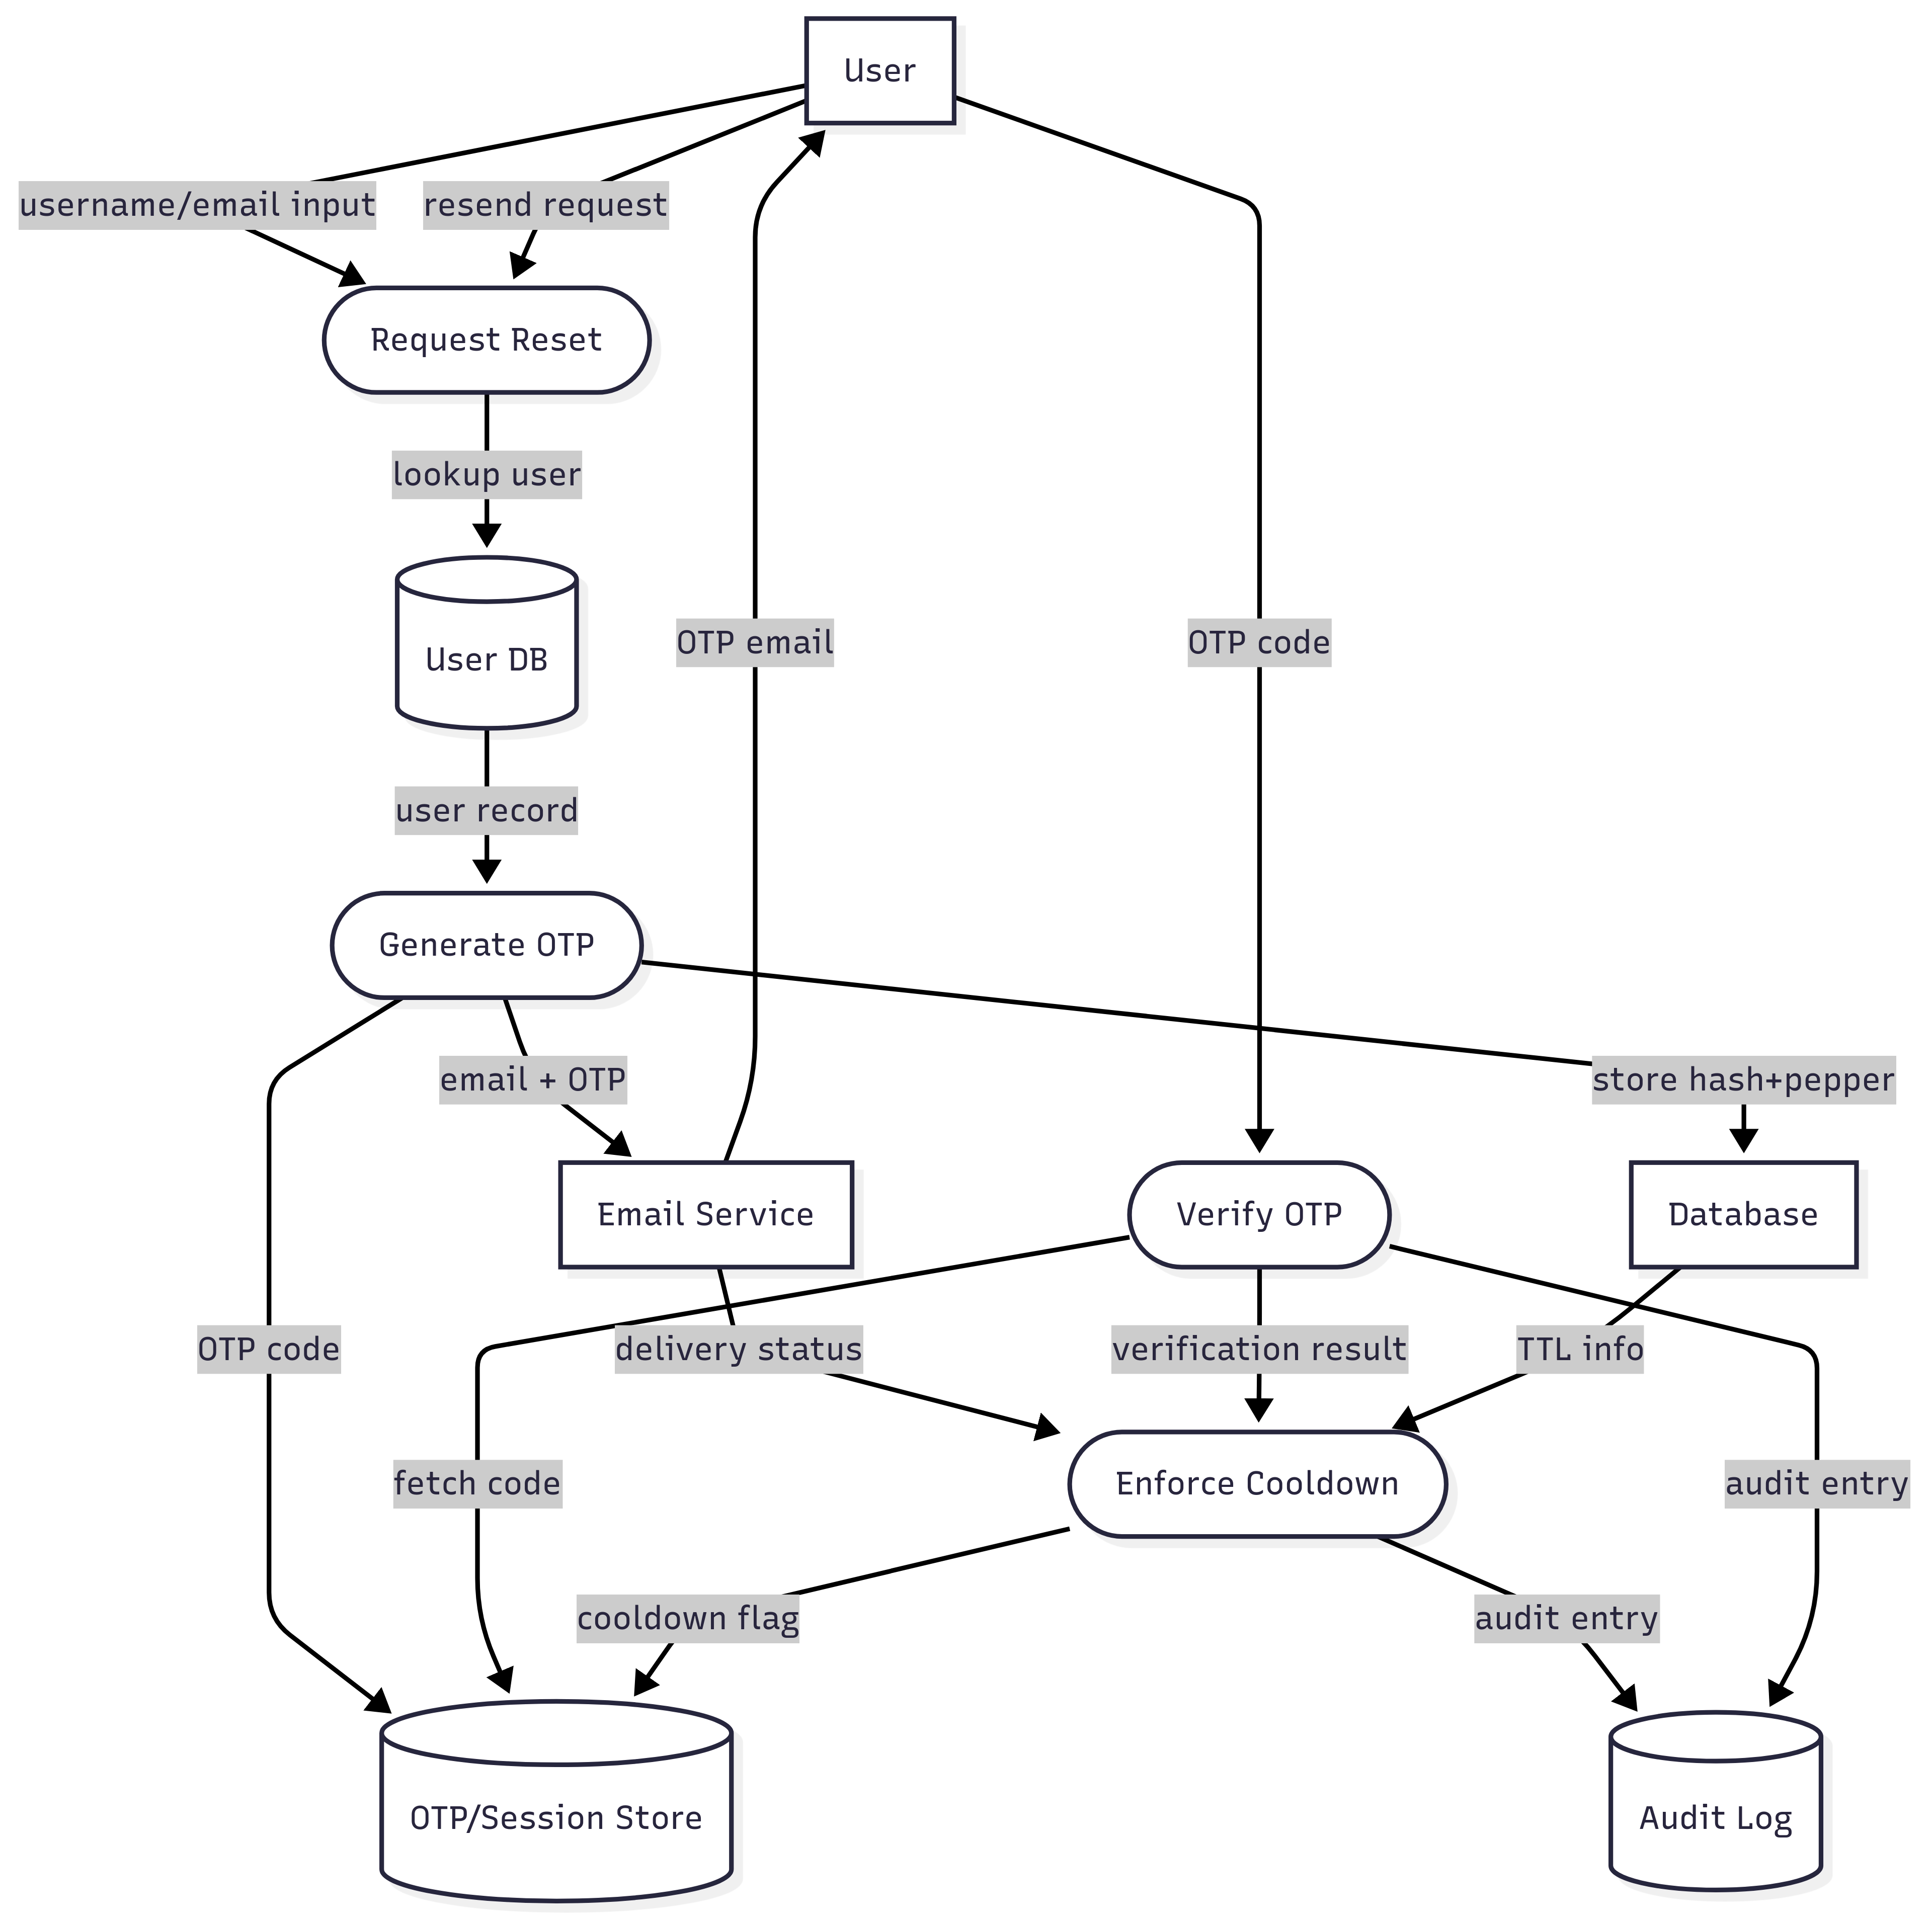
\includegraphics[width=0.9\linewidth]{detailed_data_flow.png}
  \caption{OTP verification data-flow highlighting storage boundaries and audit trails.}
  \label{fig:dfd}
\end{figure}

\section{Experimental Evaluation}
A 70/30 stratified split is employed for training and testing. Table~\ref{tab:metrics} summarizes held-out performance metrics. XGBoost attains marginal gains in accuracy and recall over the Random Forest baseline, reducing both false positives and negatives. Calibration curves exhibit near-diagonal alignment, and the area under the ROC curve exceeds 0.95 for both models.

\begin{table}[t]
  \caption{Held-Out Performance Metrics}
  \label{tab:metrics}
  \centering
  \begin{tabular}{lcccc}
    \toprule
    Model & Accuracy & Precision & Recall & F1-score \\
    \midrule
    Random Forest & 0.912 & 0.93 & 0.91 & 0.92 \\
    XGBoost & 0.920 & 0.94 & 0.92 & 0.93 \\
    \bottomrule
  \end{tabular}
\end{table}

Error analysis indicates that misclassifications predominantly occur in borderline cases with ambiguous chest pain and normal cholesterol levels, suggesting value in augmenting the dataset with imaging or longitudinal biomarkers. Fairness audits reveal a 4\% disparity in recall between sexes, motivating future bias mitigation strategies.

\section{Discussion}
Integrating visualization, modeling, and security yields tangible benefits: clinicians receive interpretable risk stratification, administrators observe policy compliance, and patients gain confidence through privacy-preserving account recovery. The modular design supports continuous retraining and policy updates without sacrificing traceability.

\section{Conclusion and Future Work}
Heartlytics demonstrates that machine-learning-driven screening can coexist with rigorous security practices. Future work will pursue (i) federated learning to leverage multi-institutional data without centralization, (ii) sensitivity-tuned alerting for high-risk cohorts, (iii) differential privacy for audit logs, and (iv) deployment on zero-trust Kubernetes meshes to isolate critical services.

\section*{Acknowledgment}
The authors thank the contributors to the Heartlytics project for data engineering, visualization, and platform hardening support.

\begin{thebibliography}{1}
\bibitem{breiman2001random} L.~Breiman, ``Random forests,'' \emph{Machine Learning}, vol.~45, no.~1, pp.~5--32, 2001.
\bibitem{chen2016xgboost} T.~Chen and C.~Guestrin, ``XGBoost: A scalable tree boosting system,'' in \emph{Proceedings of the 22nd ACM SIGKDD International Conference on Knowledge Discovery and Data Mining}, 2016, pp.~785--794.
\bibitem{zhang2021heart} D.~Zhang \emph{et~al.}, ``Heart disease prediction based on the embedded feature selection method and deep neural network,'' \emph{Journal of Healthcare Engineering}, 2021.
\bibitem{janosi1988uci} A.~Janosi, W.~Steinbrunn, M.~Pfisterer, and R.~Detrano, ``Heart disease dataset,'' UCI Machine Learning Repository, 1988.
\bibitem{flaskdocs} A.~Ronacher, ``Flask documentation,'' Pallets Projects, 2021. [Online]. Available: \url{https://flask.palletsprojects.com}
\bibitem{provos1999bcrypt} N.~Provos and D.~Mazieres, ``Bcrypt adaptive hash function,'' in \emph{USENIX Technical Report}, 1999.
\end{thebibliography}

\end{document}
